% Options for packages loaded elsewhere
\PassOptionsToPackage{unicode}{hyperref}
\PassOptionsToPackage{hyphens}{url}
\PassOptionsToPackage{dvipsnames,svgnames,x11names}{xcolor}
%
\documentclass[
  letterpaper,
  DIV=11,
  numbers=noendperiod]{scrartcl}

\usepackage{amsmath,amssymb}
\usepackage{lmodern}
\usepackage{iftex}
\ifPDFTeX
  \usepackage[T1]{fontenc}
  \usepackage[utf8]{inputenc}
  \usepackage{textcomp} % provide euro and other symbols
\else % if luatex or xetex
  \usepackage{unicode-math}
  \defaultfontfeatures{Scale=MatchLowercase}
  \defaultfontfeatures[\rmfamily]{Ligatures=TeX,Scale=1}
\fi
% Use upquote if available, for straight quotes in verbatim environments
\IfFileExists{upquote.sty}{\usepackage{upquote}}{}
\IfFileExists{microtype.sty}{% use microtype if available
  \usepackage[]{microtype}
  \UseMicrotypeSet[protrusion]{basicmath} % disable protrusion for tt fonts
}{}
\makeatletter
\@ifundefined{KOMAClassName}{% if non-KOMA class
  \IfFileExists{parskip.sty}{%
    \usepackage{parskip}
  }{% else
    \setlength{\parindent}{0pt}
    \setlength{\parskip}{6pt plus 2pt minus 1pt}}
}{% if KOMA class
  \KOMAoptions{parskip=half}}
\makeatother
\usepackage{xcolor}
\setlength{\emergencystretch}{3em} % prevent overfull lines
\setcounter{secnumdepth}{-\maxdimen} % remove section numbering
% Make \paragraph and \subparagraph free-standing
\ifx\paragraph\undefined\else
  \let\oldparagraph\paragraph
  \renewcommand{\paragraph}[1]{\oldparagraph{#1}\mbox{}}
\fi
\ifx\subparagraph\undefined\else
  \let\oldsubparagraph\subparagraph
  \renewcommand{\subparagraph}[1]{\oldsubparagraph{#1}\mbox{}}
\fi


\providecommand{\tightlist}{%
  \setlength{\itemsep}{0pt}\setlength{\parskip}{0pt}}\usepackage{longtable,booktabs,array}
\usepackage{calc} % for calculating minipage widths
% Correct order of tables after \paragraph or \subparagraph
\usepackage{etoolbox}
\makeatletter
\patchcmd\longtable{\par}{\if@noskipsec\mbox{}\fi\par}{}{}
\makeatother
% Allow footnotes in longtable head/foot
\IfFileExists{footnotehyper.sty}{\usepackage{footnotehyper}}{\usepackage{footnote}}
\makesavenoteenv{longtable}
\usepackage{graphicx}
\makeatletter
\def\maxwidth{\ifdim\Gin@nat@width>\linewidth\linewidth\else\Gin@nat@width\fi}
\def\maxheight{\ifdim\Gin@nat@height>\textheight\textheight\else\Gin@nat@height\fi}
\makeatother
% Scale images if necessary, so that they will not overflow the page
% margins by default, and it is still possible to overwrite the defaults
% using explicit options in \includegraphics[width, height, ...]{}
\setkeys{Gin}{width=\maxwidth,height=\maxheight,keepaspectratio}
% Set default figure placement to htbp
\makeatletter
\def\fps@figure{htbp}
\makeatother

\KOMAoption{captions}{tableheading}
\makeatletter
\makeatother
\makeatletter
\makeatother
\makeatletter
\@ifpackageloaded{caption}{}{\usepackage{caption}}
\AtBeginDocument{%
\ifdefined\contentsname
  \renewcommand*\contentsname{Table of contents}
\else
  \newcommand\contentsname{Table of contents}
\fi
\ifdefined\listfigurename
  \renewcommand*\listfigurename{List of Figures}
\else
  \newcommand\listfigurename{List of Figures}
\fi
\ifdefined\listtablename
  \renewcommand*\listtablename{List of Tables}
\else
  \newcommand\listtablename{List of Tables}
\fi
\ifdefined\figurename
  \renewcommand*\figurename{Figure}
\else
  \newcommand\figurename{Figure}
\fi
\ifdefined\tablename
  \renewcommand*\tablename{Table}
\else
  \newcommand\tablename{Table}
\fi
}
\@ifpackageloaded{float}{}{\usepackage{float}}
\floatstyle{ruled}
\@ifundefined{c@chapter}{\newfloat{codelisting}{h}{lop}}{\newfloat{codelisting}{h}{lop}[chapter]}
\floatname{codelisting}{Listing}
\newcommand*\listoflistings{\listof{codelisting}{List of Listings}}
\makeatother
\makeatletter
\@ifpackageloaded{caption}{}{\usepackage{caption}}
\@ifpackageloaded{subcaption}{}{\usepackage{subcaption}}
\makeatother
\makeatletter
\@ifpackageloaded{tcolorbox}{}{\usepackage[many]{tcolorbox}}
\makeatother
\makeatletter
\@ifundefined{shadecolor}{\definecolor{shadecolor}{rgb}{.97, .97, .97}}
\makeatother
\makeatletter
\makeatother
\ifLuaTeX
  \usepackage{selnolig}  % disable illegal ligatures
\fi
\IfFileExists{bookmark.sty}{\usepackage{bookmark}}{\usepackage{hyperref}}
\IfFileExists{xurl.sty}{\usepackage{xurl}}{} % add URL line breaks if available
\urlstyle{same} % disable monospaced font for URLs
\hypersetup{
  colorlinks=true,
  linkcolor={blue},
  filecolor={Maroon},
  citecolor={Blue},
  urlcolor={Blue},
  pdfcreator={LaTeX via pandoc}}

\author{}
\date{}

\begin{document}
\ifdefined\Shaded\renewenvironment{Shaded}{\begin{tcolorbox}[borderline west={3pt}{0pt}{shadecolor}, sharp corners, enhanced, breakable, interior hidden, boxrule=0pt, frame hidden]}{\end{tcolorbox}}\fi

For each of the following problems, provide your answer and show the
steps taken to solve the problem.

Problem 1. Maximum Likelihood Estimation (50 points) Given a dataset
\{x1, x2, \ldots, xN \} of size N, derive the maximum likelihood
estimate (as a function of x1, \ldots, xN ) for: (a) The lower and upper
limits, a and b, of a uniform distribution,

f(x; a, b) = \left\{

\begin{array}{ll}
\frac{1}{b-a}, & \text{if } a \leq x \leq b \\
0, & \text{otherwise}
\end{array}

\begin{enumerate}
\def\labelenumi{(\arabic{enumi})}
\tightlist
\item
\end{enumerate}

(assuming each xi ∈ R). Show all of your work. (25 points)

to find the upper limit of a uniform distribution we have:

\[ b_{MLE} = argmax P_{b}(x_{1}, x_{2}, ... , x_{N}) \]
\[ = argmax \prod_{i=1}^{N} \frac{1}{b-a} \]

\[ = argmax (\frac{1}{b-a})^N \]

From this expression we can see that the larger \(b\), the larger the
maximum likelihood estimation. Therefore, we can conclude that \$b =
max(x\_\{i\}) \$

Similarly for the lower limit,

\[ a_{MLE} = argmax P_{a}(x_{1}, x_{2}, ... , x_{N}) \]
\[ = argmax \prod_{i=1}^{N} \frac{1}{b-a} \]

\[ = argmax (\frac{1}{b-a})^N \]

The smaller \(a\) the larger the MLE, Therefore, we can conclude that
\(a = min(x_{i})\)

To test this, we can draw the uniform distribution and some x values:

\begin{figure}

{\centering 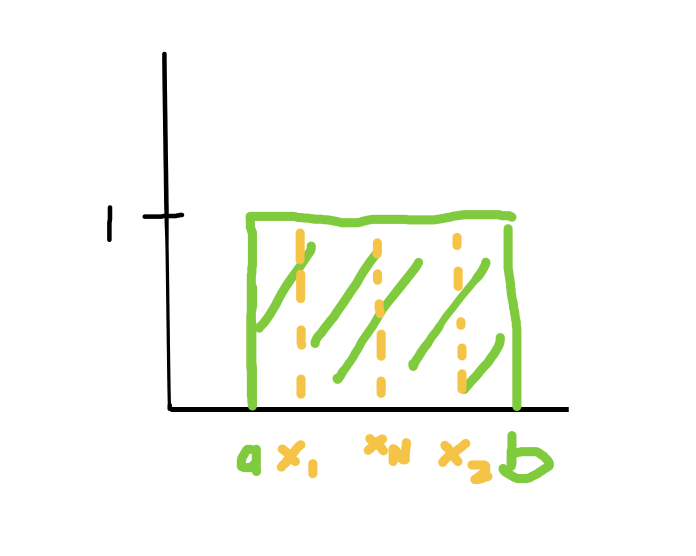
\includegraphics{./uniformDistribution.png}

}

\caption{uniform distribution}

\end{figure}

If some value of x was greater than b, the probability would be 0 and if
some value of x was less than a, the probability would also be 0.
Therefore to maximize the likelihood, we want all values of x to fall
within the range \(a\) and \(b\).

\newpage{}

\textbf{I didn't have time to finish :(}

\begin{enumerate}
\def\labelenumi{(\alph{enumi})}
\setcounter{enumi}{1}
\tightlist
\item
  The λ parameter of a Poisson distribution, f(x; λ) = ( e −λ λ x x! , x
  ≥ 0 0 x \textless{} 0
\end{enumerate}

\begin{enumerate}
\def\labelenumi{(\arabic{enumi})}
\setcounter{enumi}{1}
\tightlist
\item
\end{enumerate}

(assuming each xi ≥ 0). Show all of your work. (25 points) Hints: (i)
plotting some sample data may be helpful and calculus should not be
required (a); (ii) maximizing the log likelihood provides the same
parameter values and often provides a simpler path to a solution (b);
(iii) log(ab) = log a + log b; (iv) log e a = a.

\newpage{}

Problem 2. Bayesian Parameter Estimation (50 points) The density
function of an exponential distribution is given by fλ(x) = λe−λx. The
MLE for the parameter λ can be calculated as λ = n Σixi . We will now
consider Bayesian parameter estimation for this distribution.

\begin{enumerate}
\def\labelenumi{(\alph{enumi})}
\tightlist
\item
  Using a prior distribution from the Gamma distribution, fα,β(λ) = β αλ
  α−1 e −λβ Γ(α) , with parameters α and β, show that the posterior
  distribution for λ, after updating using three datapoints x1, x2, x3,
  is also a Gamma distribution and show its new parameter values, α 0
  and β 0 , in terms of α, β, x1, x2, and x3. (25
\end{enumerate}

points)

\newpage{}

\begin{enumerate}
\def\labelenumi{(\alph{enumi})}
\setcounter{enumi}{1}
\tightlist
\item
  If our prior parameters are α = 2 and β = 1, and our data sample
  consists of x1 = 3.7, x2 = 4.5, x3 = 4.8: Compute the posterior
  probability of a new datapoint x4 = 3.8 under the fully Bayesian
  estimation of λ. You can either leave your answer in terms of the
  Gamma function, or provide the exact answer. (13 points) Hints: (i)
  You shouldn't have to solve the complicated integral; (ii) Since the
  Gamma distribution normalizes to 1, R λ λ α−1 e −λβdλ = Γ(α) βα ;
  (iii) The Gamma function is related to the factorial function as
\end{enumerate}

Γ(x) = (x − 1)! for positive integers x.

\newpage{}

\begin{enumerate}
\def\labelenumi{(\alph{enumi})}
\setcounter{enumi}{2}
\tightlist
\item
  If we have the same prior and datapoints as in (b), what is the
  probability of a new datapoint x4 = 3.8 using maximum a posteriori
  estimation of λ? (12 points) Hint: (i) The mode of the Gamma
  distribution (i.e., the λ that attains its maximal probability) is α−1
\end{enumerate}



\end{document}
